\chapter[Practical Hybrid Quantum-Classical Computing]{Practical Hybrid Quantum-Classical\\Computing} \label{chap:practical-hybrid-quantum-classical-computing}
This chapter is focused on the practical execution of \glspl{hqca} using the Quantum Inspire quantum computing platform and SURF's \gls{hpc} center.
It gives a description of the relevant systems involved

\section{Quantum Inspire}
Quantum Inspire is a full-stack quantum computing platform that QuTech launched last year to make quantum systems available to the general public for exploratory research~\cite{last2020quantum}.
Users can run quantum circuits on different back-ends through the Quantum Inspire web editor or by using the Python \gls{sdk}.
The \gls{cqasm}~\cite{khammassi2018cqasm} is used for describing quantum circuits, but the popular quantum computing frameworks ProjectQ~\cite{steiger2018projectq} and Qiskit~\cite{qiskit} are also supported by the Python \gls{sdk}.
Quantum Inspire supports the execution of quantum circuits on real quantum chips and through quantum simulation.
An overview of the Quantum Inspire workflow and available device back-ends is shown in \Cref{fig:qi-workflow}.

The two available quantum chips are Starmon-5 and Spin-2 which have five and two qubits respectively.
These chips suffer from noise, limited coherence time, limited qubit connectivity, and each quantum chip has a specific allowed gate set.
Note that these gate sets are universal, and non-native gates are decomposed into supported gates depending on the chip.
Regardless of the limitations of these quantum chips, they are an essential part in research towards better quantum hardware and quantum algorithms.
\begin{figure}[ht]
    \centering
    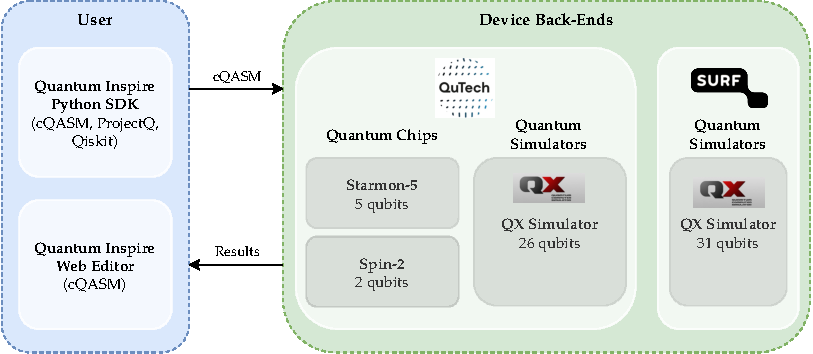
\includegraphics[width=1\linewidth]{figures/qi-workflow.pdf}
    \caption[Overview of the Quantum Inspire workflow.]{
        Overview of the Quantum Inspire workflow.
        Users can submit quantum circuits written in \gls{cqasm} using the web editor or Python \gls{sdk}.
        After the program has been run, the results are returned to the user.
        The quantum circuit can be executed on one of the quantum chips or simulated using one of the QX simulator back-ends.
        QuTech's simulator back-end supports simulations up to 26 qubits, while SURF's simulator back-end supports simulations up to 31 qubits.
    }
    \label{fig:qi-workflow}
\end{figure}

In the absence of large-scale and fault-tolerant quantum computers, quantum computer simulation is critical for developing and testing quantum algorithms.
Quantum Inspire offers two simulator back-ends which use QX~\cite{khammassi2017qx} as quantum computer simulator.
One of the simulator back-ends is hosted by QuTech on a commodity cloud-based server with 4GB of RAM, which can run simulations up to 26 qubits.
The other simulator back-end is hosted on SURF's cluster computer Lisa which consists of several hundreds of multi-core nodes.
The largest node available on Lisa has 256GB of RAM, which supports simulations up to 31 qubits.

When quantum circuits are submitted to Quantum Inspire, they are handed to a job scheduler which will attempt to schedule the job as quickly as possible when the requested resources are available.
For the quantum chips and QuTech simulator back-ends, the jobs are simply placed in a queue which are executed in first-in-first-out order.

\section{SURF High Performance Computing}

\section{Implementation}